\chapter{Extending the TBox}
\label{chap:tbox}

In this chapter you will:
\begin{enumerate}
\item Just add lots of defined classes for all the aspects we have covered in this \fhkb tutorial;
\item You will learn that the properties used in these defined classes must be chosen with care.
\end{enumerate}

\snapshot{There is a snapshot of the ontology as required at this point in the tutorial available at \fhkbhome.}

\section{Adding Defined Classes}

%\todo{Normalize class names in the following, whitespace, capitalisation}
Add the following defined classes:
\steps{Adding defined classes}{
\item Relation and blood relation;
\item Forefather and Foremother;
\item Grandparent, Grandfather and Grandmother;
\item GreatGrandparent, GreatGrandfather and GreatGrandmother;
\item GreatGrandparentOfRobert, GreatGrandfatherOfRobert and  GreatGrandMotherOfRobert
\item Daughter, Son, Brother, Sister, Child;
\item Aunt, Uncle, AuntInLaw, UncleInLaw, GreatAunt and GreatUncle; %removed great aunt great uncle
\item FirstCousin and SecondCousin;
\item First cousin once removed;
\item InLaw, MotherInLaw, FatherInLaw, ParentInLaw, SiblingInLaw, SisterInLaw, BrotherInLaw;
\item Any defined class for any property in the hierarchy and any nominal variant of these classes.
}

The three classes of \con{Child}, \con{Son} and \con{Daughter} are of note. They are coded in the following way:

\owlcode{
Class: Child
	EquivalentTo: Person
		that hasParent Some Person

Class: Son
	EquivalentTo: Man
		that hasParent Some Person

Class: Daughter
	EquivalentTo: Woman
		that hasParent Some Person
}

After running the reasoner, you will find that \con{Person} is found to be equivalent to \con{Child}; \con{Daughter} is equivalent to \con{Woman} and that \con{Son} is equivalent to \con{Man}. This does, of course, make sense -- each and every person is someone's child, each and every woman is someone's daughter. We will forget evolutionary time-scales where this might be thought to break down at some point -- all \con{Person} individuals are also \con{Descendant} individuals, but do we expect some molecule in some prebiotic soup to be a member of this class?

Nevertheless, within the scope of the \fhkb, such inferred equivalences are not unreasonable. They are also instructive; it is possible to have different intentional descriptions of a class and for them to have the same logical extents. You can see another example of this happening in the amino acids ontology, but for different reasons.

Taking \con{Grandparent} as an example class, there are two ways of writing the defined class:

\owlcode{
Class: Grandparent
	EquivalentTo: Person
		and isGrandparentOf some Person

Class: Grandparent
	EquivalentTo: Person
	and (isParentOf some (Person and (isParentOf some Person))
}

Each comes out at a different place in the class hierarchy. They both capture the right individuals as members (that is, those individuals in the ABox that are holding a \con{isGrandparentOf} property), but the class hierarchy is not correct. By definition, all grandparents are also parents, but the way the object property hierarchy works means that the first way of writing the defined class (with the \con{isGrandparentOf} property) is not subsumed by the class \con{Parent}. We want this to happen in any sensible class hierarchy, so we have to use the second pattern for all the classes, spelling out the sub-property path that implies the property such as \con{isGrandparentOf} within the equivalence axiom.

The reason for this need for the `long-form' is that the \con{isGrandparentOf} does not imply the \con{isParentOf} property. As described in Chapter~\ref{chap:ancestor} if this implication were the case, being a grandparent of \rds, for instance, would also imply that the same \person were a parent of \rds; an implication we do not want. As these two properties (\con{isParentOf} and \con{isGrandparentOf}) do not subsume each other means that the defined classes written according to pattern one above will not subsume each other in the class hierarchy. Thus we use the second pattern.
If we look at the class for grandparents of Robert:

\owlcode{
Class: GrandparentOfRobert

EquivalentTo: Person
		that isParentOf some (Person
			that isParentOf value \rds)
}

If we make the equivalent class for \rjs, apply the reasoner and look at the hierarchy, we see that the two classes are not logically equivalent, even though they have the same extents of William George Bright, Iris Ellen Archer, Charles Herbert Rever and Violet Sylvia Steward. We looked at this example in Section~\ref{sec:nom_owa}, where there is an explanation and solutions.

\begin{figure}
\begin{center}
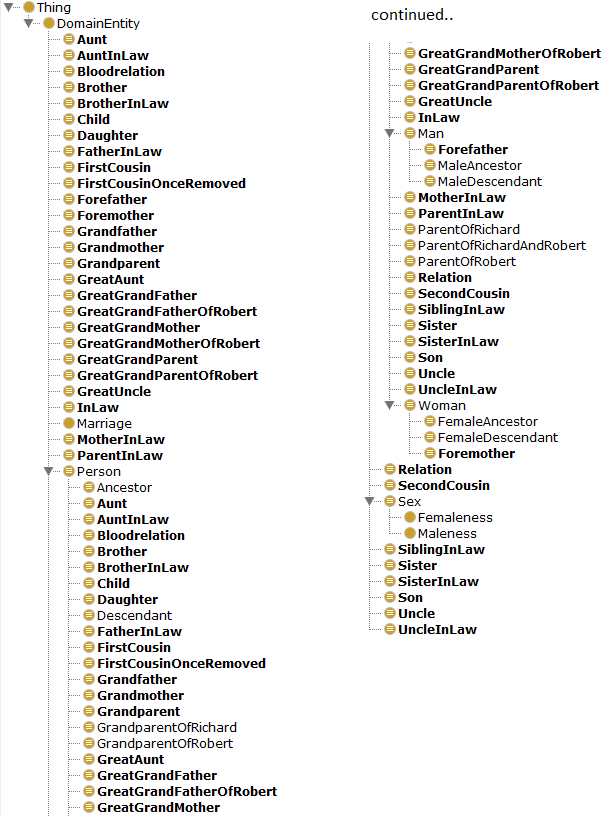
\includegraphics[width=\largefigwidth]{figures/class_hierachy_final_1}\caption{The full TBox hierarchy of the \fhkb}
\label{fig:tbox2}
\end{center}
\end{figure}

\section{Summary}

We can add defined classes based on each property we have put into the object property hierarchy. We see the expected hierarchy; as can be seen from Figure~\ref{fig:tbox2} it has an obvious symmetry based on sex. We also see a lot of equivalences inferred -- all women are daughters, as well as women descendants. Perhaps not the greatest insight ever gained, but it at least makes sense; all women must be daughters. It is instructive to use the explanation feature in \protege to look at why the reasoner has made these inferences. For example, take a look at the class \con{hasGrandmother some Woman} -- it is instructive to see how many there are.

Like the Chapter on marriage and in-law (Chapter~\ref{chap:marriage}), this chapter has largely been revision. One thing of note is, however, that we must not use the object properties that are inferred through sub-property chains as definitions in the TBox; we must spell out the sub-property chain in the definition, otherwise the implications do not work properly.

One thing is almost certain; the resulting TBox is rather complex and would be almost impossible to maintain by hand.
\\
\expressivity{SROIQ(D)}

\ctime{0}{0}{35438}